\chapter{Implementacija i korisničko sučelje}
		
		
		\section{Korištene tehnologije i alati}
		
		Za komunikaciju medu clanovima tima smo koristili discord\footnote{\url{https://discord.com/download}}i whatsapp\footnote{\url{https://www.whatsapp.com/download}}.
		Za izradu Uml dijagrama korisitli smo Astah\footnote{\url{https://astah.net/products/astah-professional/}}.
		Za upravljanje izvornim kodom koristili smo Git\footnote{\url{https://git-scm.com/downloads}}, a udaljeni repozitorij nalazio se na GitLabu\footnote{\url{https://about.gitlab.com/install/}}.
		
		Razvojno okruzenje nam je bio Intellij\footnote{\url{https://www.jetbrains.com/idea/download}}.
		Diffblue Cover\footnote{\url{https://www.diffblue.com/products/}} koji generira testove za ispitivanje koda po komponentama. 
		IntelliJ IDEA je integrirano razvojno okruženje (IDE) napisano u Javi za razvoj računalnog softvera. 
		Razvio ga je JetBrains (prije poznat kao IntelliJ), a dostupan je besplatno preko licence za studente za koju smo se prijavili sa FER-ovim mailom.
		
		Web aplikaciju smo napisali u Javi\footnote{\url{https://www.java.com/download/ie_manual.jsp}} koristeci Spring Boot\footnote{\url{https://spring.io/projects/spring-boot}} framework za izradu backenda, a thymeleaf\footnote{\url{https://www.thymeleaf.org/}}, html, css i javascript\footnote{\url{https://www.javascript.com/}} za izradu frontenda.
		
		Spring Boot je open-source framework koji održava tvrtka pod nazivom Pivotal. Pruža Java programerima platformu za početak rada s aplikacijom koja se može automatski konfigurirati.
		
		Thymeleaf je Java teamplate engine koji omogucuje rad sa HTML, XML, JavaScript i CSS datotekama.
			\eject 
		
	
		\section{Ispitivanje programskog rješenja}
			
			
			 Testove smo izvodili na strukturirani nacin pomocu selenium testova.
			  Ispitivanje se radilo po obrascima uporabe kako bi se provjerila osnovna funkcionalnost sustava, ali i nasumicnim kretanjima po 
			  aplikaciji kako bi se pronasle neocekivane greske  ili nepredvidena ponasanja.			  
			
			\subsection{Ispitivanje komponenti}
			Ispitivanje komponenti smo radili uz pomoc plugina za IntelliJ Diffblue Cover koji generira testove za ispitivanje koda po komponentama.
			\begin{figure}[H]
				
				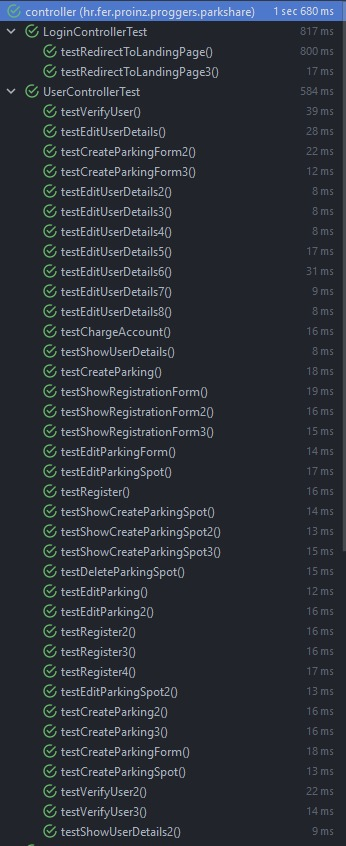
\includegraphics[width=0.5\textwidth]{slike/testovi1.jpeg} %veličina slike u odnosu na originalnu datoteku i pozicija slike
				\centering
				\caption{Testovi 1}
				\label{fig:testovi1}
			\end{figure}
		\begin{figure}[H]
			
			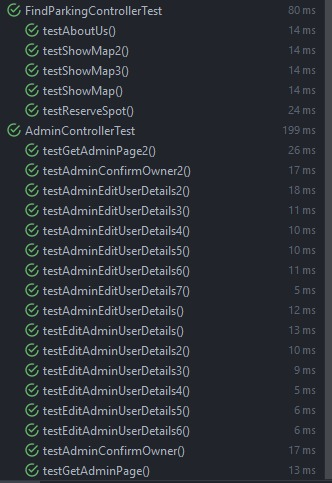
\includegraphics[width=0.5\textwidth]{slike/testovi2.jpeg} %veličina slike u odnosu na originalnu datoteku i pozicija slike
			\centering
			\caption{Testovi 2}
			\label{fig:testovi2}
		\end{figure}
			
			
			\subsection{Ispitivanje sustava}
			
			 \textit{Potrebno je provesti i opisati ispitivanje sustava koristeći radni okvir Selenium\footnote{\url{https://www.seleniumhq.org/}}. Razraditi \textbf{minimalno 4 ispitna slučaja} u kojima će se ispitati redovni slučajevi, rubni uvjeti te poziv funkcionalnosti koja nije implementirana/izaziva pogrešku kako bi se vidjelo na koji način sustav reagira kada nešto nije u potpunosti ostvareno. Ispitni slučaj se treba sastojati od ulaza (npr. korisničko ime i lozinka), očekivanog izlaza ili rezultata, koraka ispitivanja i dobivenog izlaza ili rezultata.\\ }
			 
			 \textit{Izradu ispitnih slučajeva pomoću radnog okvira Selenium moguće je provesti pomoću jednog od sljedeća dva alata:}
			 \begin{itemize}
			 	\item \textit{dodatak za preglednik \textbf{Selenium IDE} - snimanje korisnikovih akcija radi automatskog ponavljanja ispita	}
			 	\item \textit{\textbf{Selenium WebDriver} - podrška za pisanje ispita u jezicima Java, C\#, PHP koristeći posebno programsko sučelje.}
			 \end{itemize}
		 	\textit{Detalji o korištenju alata Selenium bit će prikazani na posebnom predavanju tijekom semestra.}
			
			\eject 
		
		
		\section{Dijagram razmještaja}
		
		Dijagram razmjestaja je strukturni statički UML dijagram koji opisuje topologiju sustava i usredotočen je na odnos sklopovskih i programskih dijelova.
		Imamo dijagram razmještaja, specifikacijski dijagram razmještaja, dijagram razmještaja instanci, implementacijski dijagram i dijagram mrežne arhitekture.
			
			\begin{figure}[H]
				
				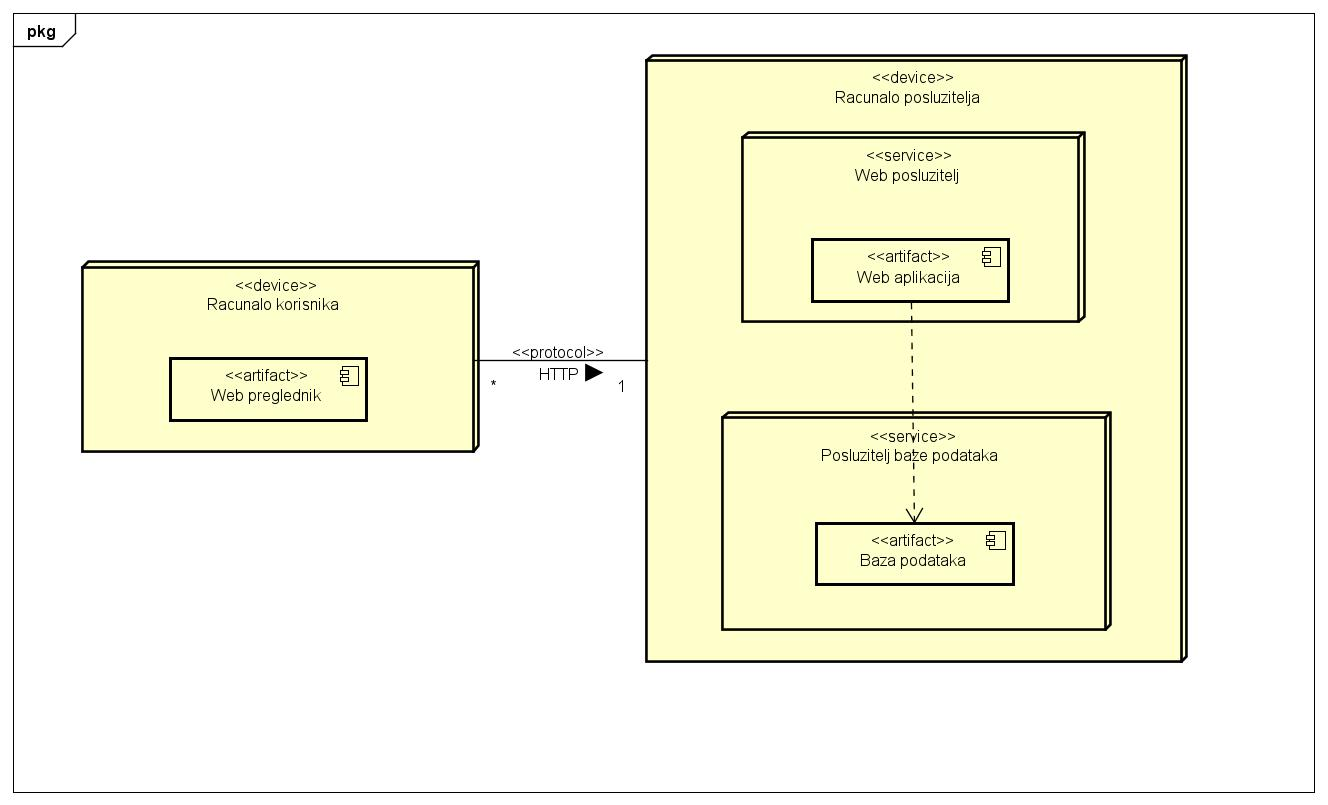
\includegraphics[width=\textwidth]{slike/Deployment Diagram0.jpg} %veličina slike u odnosu na originalnu datoteku i pozicija slike
				\centering
				\caption{Dijagram razmjestaja}
				\label{fig:dijagramraz}
			\end{figure}
			\eject 
		
		\section{Upute za puštanje u pogon}
		
		Pustanje aplikacije u pogon odradeno je koristenjem alata Heroku. Posluziteljski i klijentski dio podignuti su zasebno. Za dizanje posluziteljskog dijela pratili smo upute na stranici \footnote{\url{ https://devcenter.heroku.com/articles/deploying-spring-boot-apps-to-heroku}}.
		U projektu radimo s PostgreSql bazom podataka koja je podrzana na Heroku platformi. Integrira se u projekt dodavanjem Heroku Postgres Add-Onsa te se dobiju podatci za povezivanje s tom bazom koji se upisuju u application.properties u projektu.
		
		\begin{figure}[H]
			
			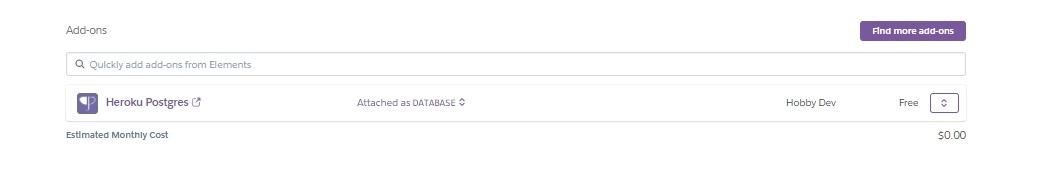
\includegraphics[width=\textwidth]{slike/prva.jpg} %veličina slike u odnosu na originalnu datoteku i pozicija slike
			\centering
			\caption{Add-Ons}
			\label{fig:addons}
		\end{figure}
	
	Prvo treba skinuti Heroku CLI(Command Line Interface) preko kojeg se koristi naredba za prijavu na Heroku. 
	Nakon toga treba pripremiti repozitorij za dizanje na Heroku koristenjem git naredbi.
	
		\begin{figure}[H]
		
		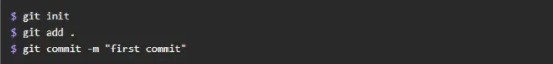
\includegraphics[width=\textwidth]{slike/druga.jpg} %veličina slike u odnosu na originalnu datoteku i pozicija slike
		\centering
		\caption{Heroku CLI}
		\label{fig:cli}
	\end{figure}
Zatim treba kreirati udaljeni Heroku repozitorij i konacno podignuti nas kod na taj repozitorij sto je prikazano na slikama 5.4 i 5.5
	\begin{figure}[H]
	
	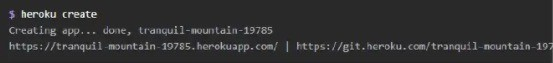
\includegraphics[width=\textwidth]{slike/treca.jpg} %veličina slike u odnosu na originalnu datoteku i pozicija slike
	\centering
	\caption{Stvaranje Heroku repozitorija}
	\label{fig:tre}
\end{figure}
\begin{figure}[H]
	
	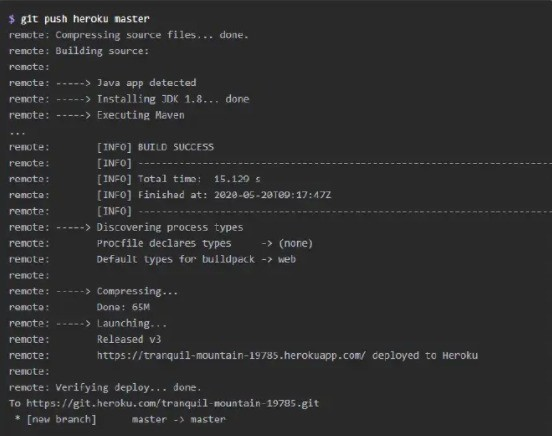
\includegraphics[width=\textwidth]{slike/cetvrta.jpg} %veličina slike u odnosu na originalnu datoteku i pozicija slike
	\centering
	\caption{Deplojanje posluziteljskog koda na Heroku}
	\label{fig:cli}
\end{figure}
Nasoj aplikaciji mozete pristupiti na linku \footnote{\url{https://park-share-proggers.herokuapp.com/}}
		
			\eject 